\subsection{2(d) Differential gear and drive shaft kinematics}
\begin{figure}[H]
    \centering
    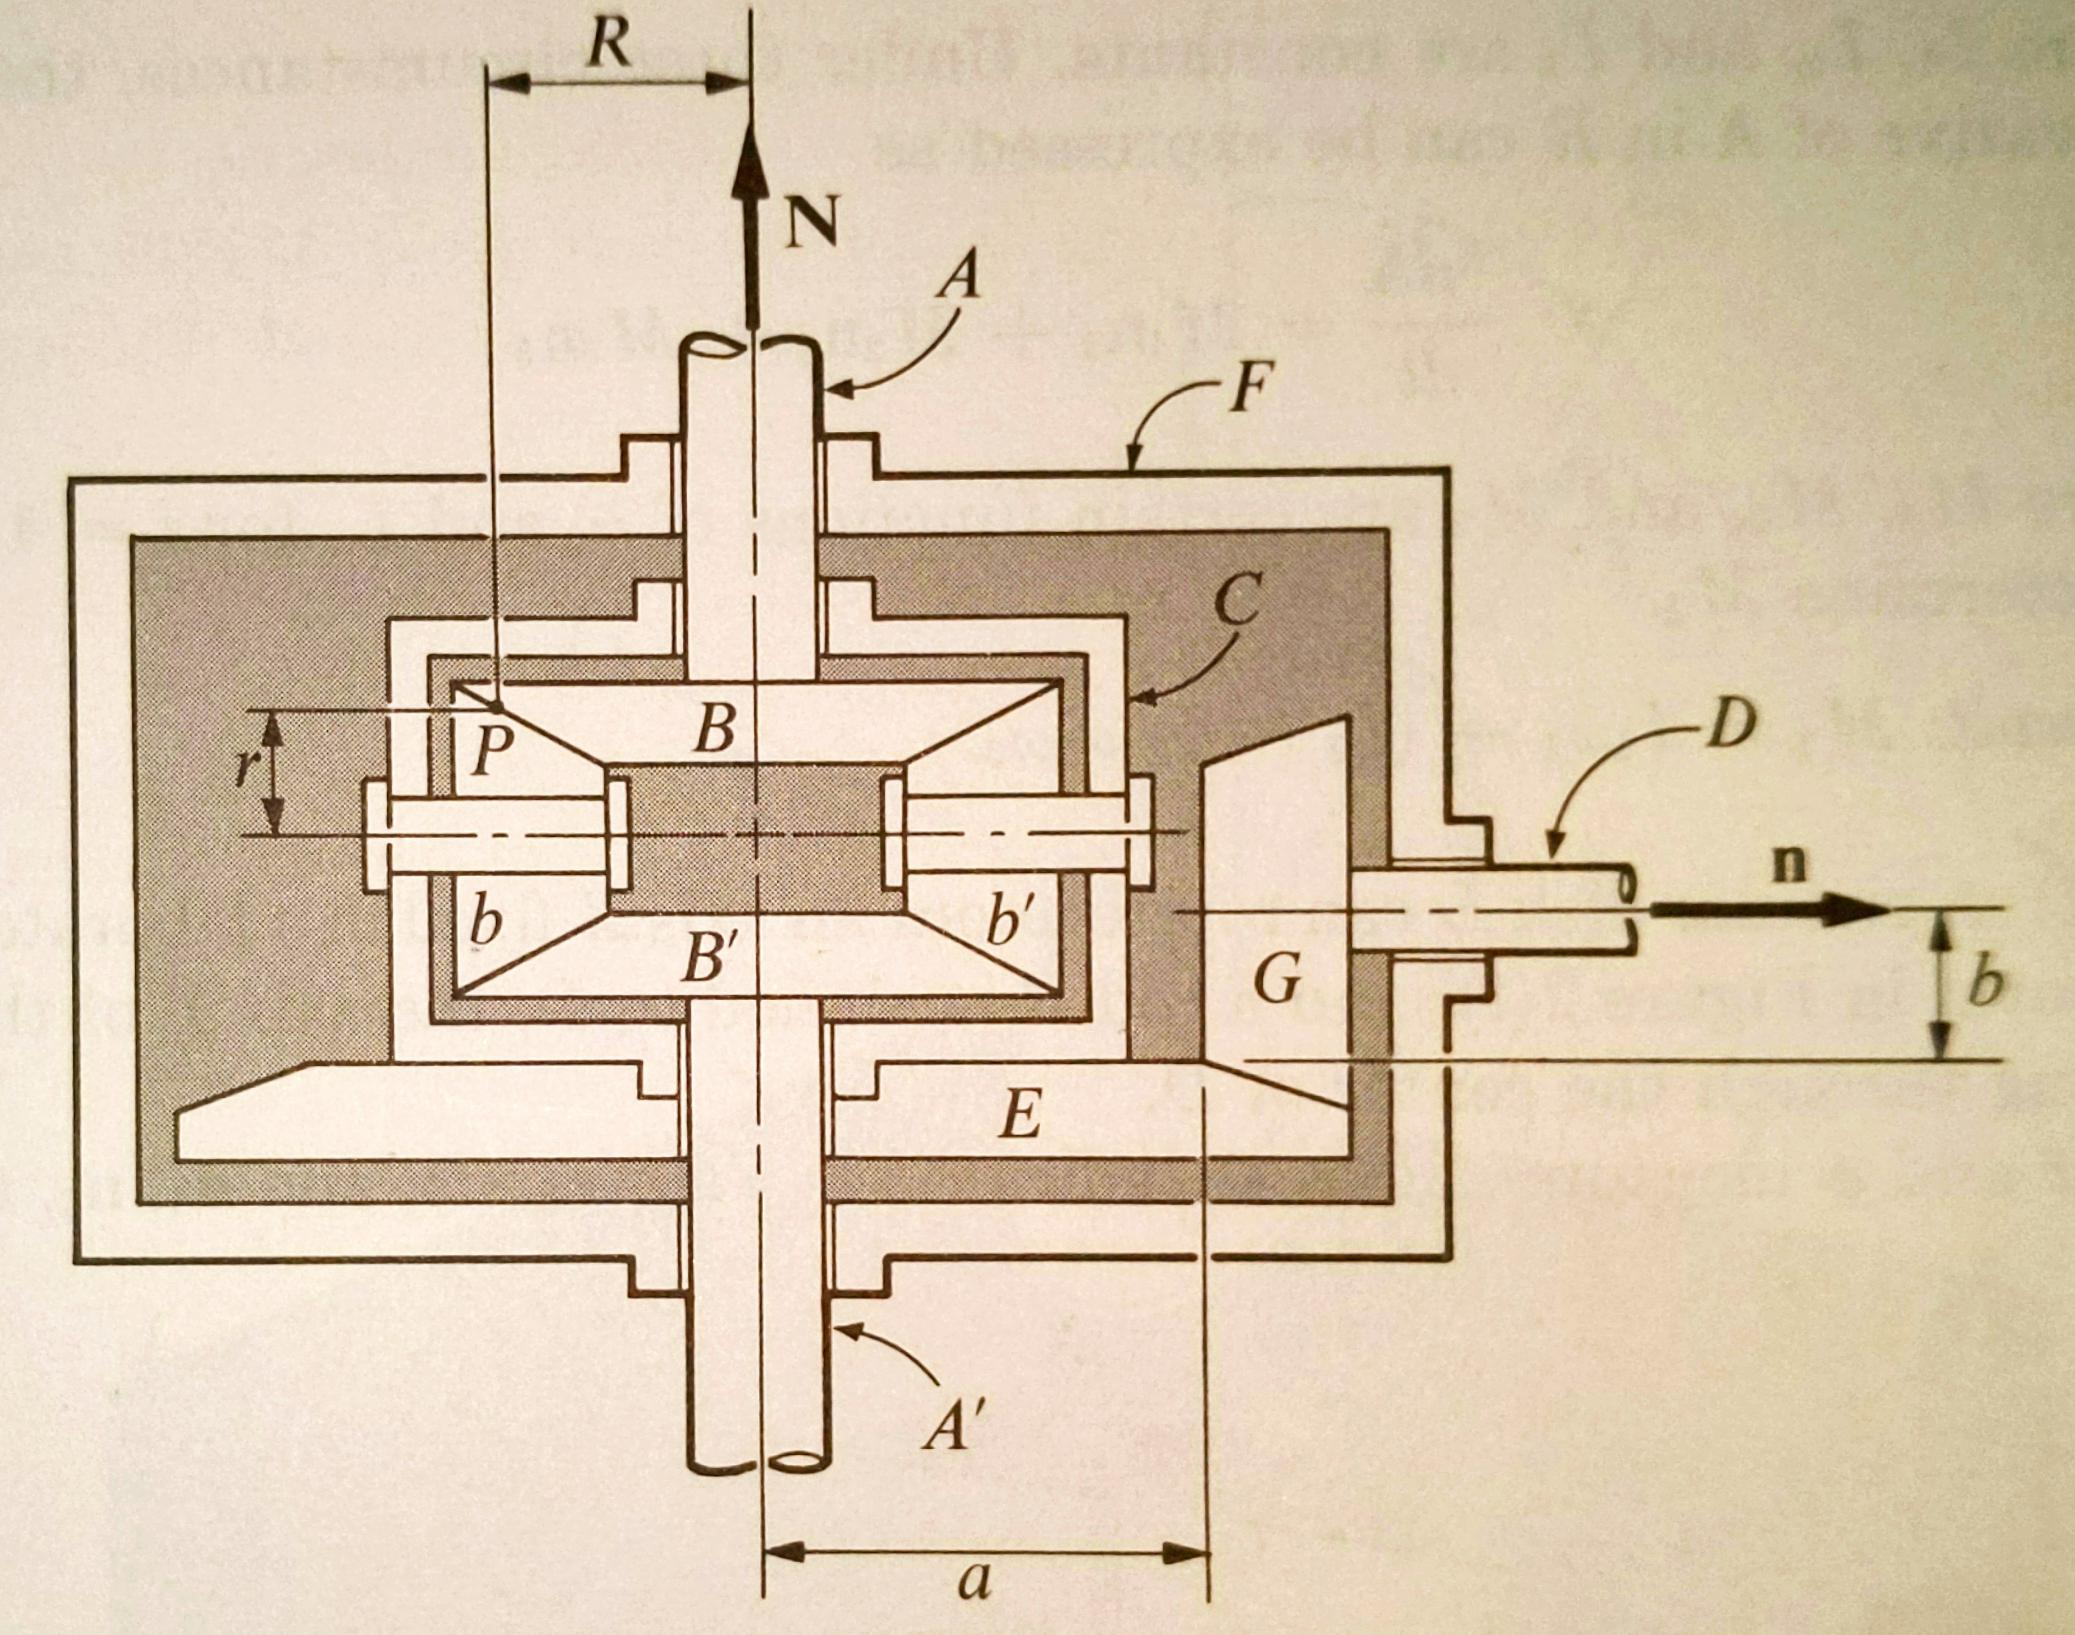
\includegraphics[scale = 0.1]{figs/ProbSet_2/2_d.jpg}
    \caption{}
    \label{2_d}
\end{figure}

\itbf{Mechanism}: Bevel gears $B$ and $B'$ are keyed to $A$ and $A'$, and engage bevel gears $b$ and $b'$, the latter being free to rotate on pins fixed in a casing $C$. $C$ can revolve about the common axis of $A$ and $A'$, and a bevel gear $E$, rigidly attached to $C$, is driven by the gear $G$, which is keyed to the drive shaft $D$.

\bigskip
Given:
\begin{align*}
    \lx{^F}{\pmb \omega}^A &= \Omega \pmb N\\
    \lx{^F}{\pmb \omega}^{A'} &=\Omega' \pmb N\\
    \lx{^F}{\pmb \omega}^D &= \omega \pmb n
\end{align*}

The gears have simple angular velocities w.r.t the frame attached to their shafts. And, the contact points should have same linear velocities. Writing only the magnitudes:
\begin{align*}
    \lx{^F}{\omega}^D b &=  \lx{^F}{\omega}^C a \implies \lx{^F}{\omega}^C  = \frac{b}{a} \omega\\
    \therefore \lx{^F}{\pmb \omega}^C  &= \frac{b}{a} \omega \pmb N\\
\end{align*}

Also,
\begin{align*}
    \lx{^C}{\pmb \omega}^B &= \lx{^F}{\pmb \omega}^B - \lx{^C}{\pmb \omega}^C
    = \lx{^F}{\pmb \omega}^A - \lx{^C}{\pmb \omega}^C = \left( \Omega - \frac{b}{a} \omega \right) \pmb N\\
    %==
     \lx{^C}{\pmb \omega}^{B'} &= \lx{^F}{\pmb \omega}^{B'} - \lx{^C}{\pmb \omega}^C
    = \lx{^F}{\pmb \omega}^{A'} - \lx{^C}{\pmb \omega}^C = \left( \Omega' - \frac{b}{a} \omega \right) \pmb N
\end{align*}

\begin{align*}
    \left . \begin{matrix}
    \lx{^C}{\omega}^{B'} R =  \lx{^C}{\omega}^{b'} r\\
    \lx{^C}{\omega}^{B'} R =  -\lx{^C}{\omega}^{b} r\\
    \lx{^C}{\omega}^{B} R =  -\lx{^C}{\omega}^{b'} r\\
    \lx{^C}{\omega}^{B} R =  \lx{^C}{\omega}^{b} r\\
    \end{matrix} \right \} &\implies \lx{^C}{\omega}^{B'} + \lx{^C}{\omega}^{B} = 0\\
    %===
    &\implies \left( \Omega - \frac{b}{a} \omega \right) + \left( \Omega' - \frac{b}{a} \omega \right) =0 \\
    %==
\end{align*}
$$ \therefore \omega = \frac{a}{2b} \left( \Omega + \Omega' \right)$$
